%======================================================================
%  Central-upwind fluxes and a PIMPLE outer loop for ICE + gasCombustion
%  Method and implementation notes.   Build:  pdflatex PIMPLE_KT_method.tex (x2)
%======================================================================
\documentclass[11pt]{article}

\usepackage[T1]{fontenc}
\usepackage[utf8]{inputenc}
\usepackage{mathpazo}
\usepackage[scaled=0.90]{helvet}
\renewcommand{\ttdefault}{lmtt}
\usepackage{microtype}
\usepackage[a4paper, margin=24mm, headheight=14pt]{geometry}
\usepackage{amsmath, amssymb, mathtools}
\usepackage{booktabs, tabularx, array}
\usepackage{enumitem}
\usepackage[dvipsnames]{xcolor}
\usepackage{tikz}
\usetikzlibrary{arrows.meta, positioning, fit, calc, decorations.pathreplacing}
\usepackage[most]{tcolorbox}
\usepackage{titlesec}
\usepackage{fancyhdr}
\usepackage[colorlinks=true, linkcolor=Ink, urlcolor=Ink, citecolor=Ink]{hyperref}

%----------------------------------------------------------------------
%  Palette
%----------------------------------------------------------------------
\definecolor{Ink}{HTML}{0B4F6C}        % deep teal: headings, links
\definecolor{Rust}{HTML}{B5532A}       % accent: deviations
\definecolor{Moss}{HTML}{4F6D3A}       % accent: code pointers
\definecolor{Paper}{HTML}{F4F1EA}      % light fill
\definecolor{Slate}{HTML}{55606B}      % secondary text

%----------------------------------------------------------------------
%  Headings: sans, teal, number hung in the margin
%----------------------------------------------------------------------
\titleformat{\section}
  {\sffamily\Large\bfseries\color{Ink}}
  {\llap{\makebox[14mm][r]{\color{Rust}\thesection\hspace{4mm}}}}{0pt}{}
  [{\color{Ink}\titlerule[0.6pt]}]
\titleformat{\subsection}
  {\sffamily\large\bfseries\color{Ink}}
  {\llap{\makebox[14mm][r]{\color{Slate}\thesubsection\hspace{4mm}}}}{0pt}{}
\titleformat{\paragraph}[runin]
  {\sffamily\bfseries\color{Ink}}{}{0pt}{}[.\ ]
\titlespacing*{\section}{0pt}{3.2ex plus 1ex}{1.6ex}
\titlespacing*{\subsection}{0pt}{2.4ex plus .8ex}{1.0ex}

\pagestyle{fancy}
\fancyhf{}
\fancyhead[L]{\sffamily\small\color{Slate} ICE $\cdot$ central-upwind fluxes $\cdot$ PIMPLE outer loop}
\fancyhead[R]{\sffamily\small\color{Slate}\thepage}
\renewcommand{\headrulewidth}{0pt}

\setlist{itemsep=2pt, topsep=4pt}
\setlength{\emergencystretch}{3em}

%----------------------------------------------------------------------
%  Callouts
%----------------------------------------------------------------------
\newtcolorbox{incode}[1][]{%
  enhanced, breakable, colback=white, colframe=Moss, boxrule=0pt,
  leftrule=2.5pt, arc=0pt, left=8pt, right=6pt, top=4pt, bottom=4pt,
  fonttitle=\sffamily\small\bfseries, coltitle=Moss, colbacktitle=white,
  attach title to upper={\ }, title={In the code#1}}
\newtcolorbox{deviation}[1][]{%
  enhanced, breakable, colback=Rust!5, colframe=Rust, boxrule=0pt,
  leftrule=2.5pt, arc=0pt, left=8pt, right=6pt, top=4pt, bottom=4pt,
  fonttitle=\sffamily\small\bfseries, coltitle=Rust, colbacktitle=Rust!5,
  attach title to upper={\ }, title={Departure from the reference#1}}
\newtcolorbox{keypoint}{%
  enhanced, colback=Paper, colframe=Paper, arc=2pt, left=10pt, right=10pt,
  top=6pt, bottom=6pt}

\newcommand{\code}[1]{\texttt{\small #1}}
\newcommand{\file}[1]{\texttt{\small\color{Moss}#1}}
\newcommand{\own}{\mathrm{own}}
\newcommand{\nei}{\mathrm{nei}}
\newcommand{\dt}{\Delta t}

\begin{document}

%======================================================================
%  Title block
%======================================================================
\thispagestyle{empty}
\begin{tikzpicture}[remember picture, overlay]
  \fill[Ink] (current page.north west) rectangle ([yshift=-58mm]current page.north east);
  \fill[Rust] ([yshift=-58mm]current page.north west) rectangle ([yshift=-60mm]current page.north east);
\end{tikzpicture}
\vspace*{-6mm}
\begingroup\color{white}\sffamily\raggedright
  {\small\bfseries UINTAH \,$\cdot$\, ICE \,$\cdot$\, gasCombustion\par}
  \vspace{5mm}
  {\LARGE\bfseries Central-upwind fluxes and a PIMPLE outer loop\par}
  \vspace{3mm}
  {\large Method and implementation notes for the \texttt{Uintah\_PIMPLE} sandbox\par}
  \vspace{2mm}
  {\small Numerics follow \emph{reactingPimpleCentralFoam} (Kraposhin et al.\ hybrid KT/PIMPLE solver)\par}
\endgroup
\vspace{20mm}

\begin{keypoint}
\textbf{\sffamily\color{Ink}In one paragraph.}
Detonations computed with ICE + gasCombustion reach the right wave speed and CJ state but
show induction zones that are too thin and oscillations right behind the shock. Two
causes were targeted. First, ICE builds face states from symmetric, centred averages that
carry no upwind dissipation. Second, a single forward-Euler stage is not TVD for limited
schemes. This work adds the Kurganov--Tadmor (KT) central-upwind flux construction of
reactingPimpleCentralFoam: limited own/nei reconstructions, local wave speeds, $\alpha$
weights, the $a_{Sf}$ dissipation term and the Mach/acoustic-Courant blending function
$\kappa$. It also adds a PIMPLE-style outer loop that re-runs the whole ICE fluid chain at
the latest iterate and combines iterates with a Crank--Nicolson $\theta$ rule. Everything
sits behind input flags that default to off; with the flags off, the original code paths
run unchanged.
\end{keypoint}

\tableofcontents
\newpage

%======================================================================
\section{Scope and the two switches}
%======================================================================

The work touches explicit ICE with a single ICE material on a single level, reacting
through the \code{gasCombustion} model. Two independent groups of options control it:

\begin{center}
\begin{tabularx}{\linewidth}{@{}l X@{}}
\toprule
\textbf{Switch} & \textbf{Effect} \\
\midrule
\code{<advection type="CentralUpwind">} &
  Turns on the KT machinery: weights, fluxes, the new advector, the KT face velocity and
  face pressure, and the KT term in the pressure update (Sections~\ref{sec:recon}--\ref{sec:press}). \\
\code{<PIMPLE> nOuterCorrectors > 1} &
  Turns on the outer loop (Section~\ref{sec:outer}). It works with any advection type but was
  designed to be paired with \code{CentralUpwind}. \\
\bottomrule
\end{tabularx}
\end{center}

\noindent
The design decisions agreed before implementation were:
\begin{itemize}
  \item \textbf{The GitHub solver is the specification for the numerics.} Earlier Uintah
        experiments were consulted only for framework plumbing (sub-scheduler data-warehouse
        handling, ghost widths).
  \item \textbf{Explicit ICE, not impICE.} pimpleCentralFoam is implicit for all-Mach
        efficiency, not for detonation stability. At the tutorial's \code{maxCo 0.1},
        $\kappa=1$ at the front and the scheme behaves like explicit KT
        (Section~\ref{sec:why-explicit}).
  \item \textbf{Energy stays in ICE's internal-energy form} with the existing
        \code{newPressWork 1} pressure work and kinetic-energy correction. No
        total-energy rewrite was made.
\end{itemize}

%======================================================================
\section{Where the changes sit in an ICE timestep}
%======================================================================

An explicit ICE step is a Lagrangian phase (pressure, face velocities, momentum and
energy sources) followed by an advection (remap) phase and a conversion back to primitive
variables. Figure~\ref{fig:flow} shows the task sequence with the new tasks marked, and
the outer loop wrapped around it.

\begin{figure}[ht]
\centering
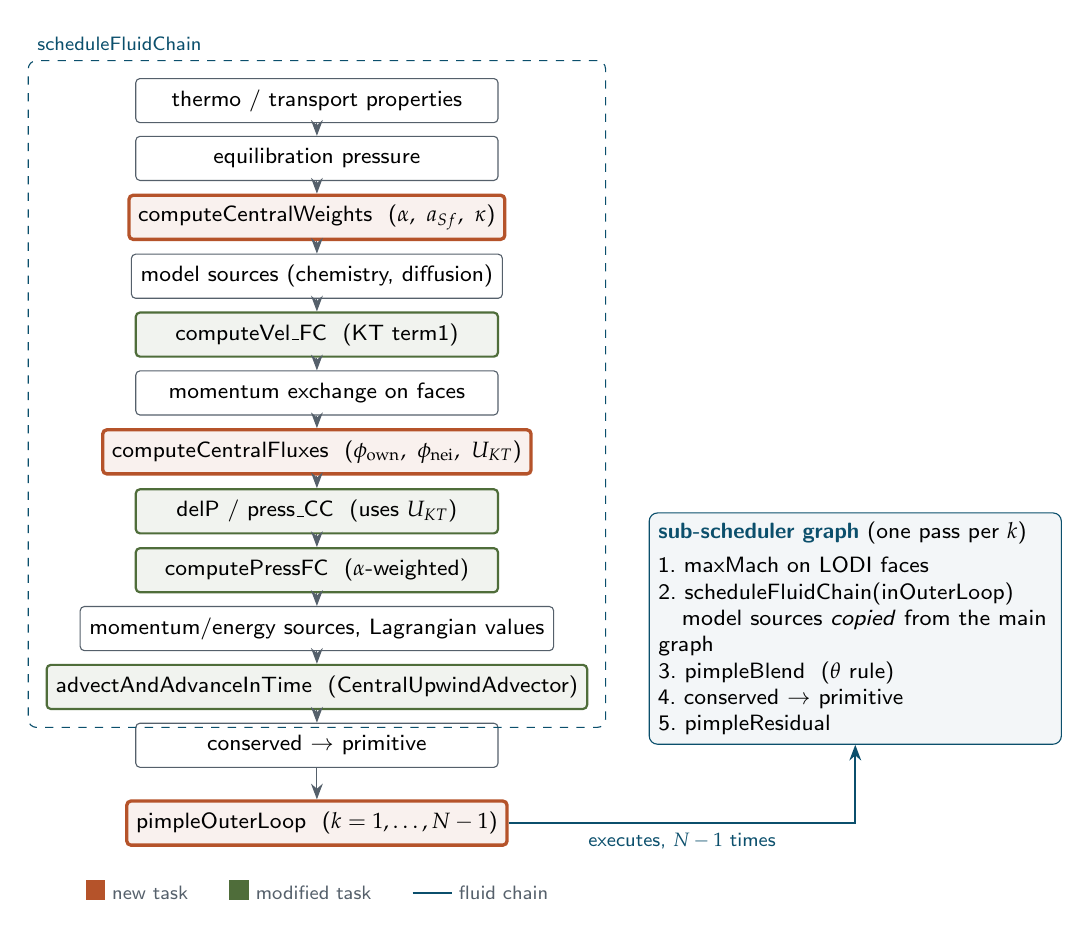
\begin{tikzpicture}[
  font=\sffamily\footnotesize,
  task/.style={draw=Slate, rounded corners=1.5pt, fill=white, minimum width=46mm,
               minimum height=5.6mm, align=center},
  new/.style={task, draw=Rust, fill=Rust!8, very thick},
  mod/.style={task, draw=Moss, fill=Moss!8, thick},
  arr/.style={-{Stealth[length=2mm]}, Slate},
  node distance=1.6mm]
  \node[task] (thermo) {thermo / transport properties};
  \node[task, below=of thermo] (eq) {equilibration pressure};
  \node[new,  below=of eq] (w) {computeCentralWeights \ ($\alpha,\ a_{Sf},\ \kappa$)};
  \node[task, below=of w] (src) {model sources (chemistry, diffusion)};
  \node[mod,  below=of src] (vfc) {computeVel\_FC \ (KT term1)};
  \node[task, below=of vfc] (ex) {momentum exchange on faces};
  \node[new,  below=of ex] (fl) {computeCentralFluxes \ ($\phi_\own,\ \phi_\nei,\ U_{KT}$)};
  \node[mod,  below=of fl] (dp) {delP / press\_CC \ (uses $U_{KT}$)};
  \node[mod,  below=of dp] (pfc) {computePressFC \ ($\alpha$-weighted)};
  \node[task, below=of pfc] (lag) {momentum/energy sources, Lagrangian values};
  \node[mod,  below=of lag] (adv) {advectAndAdvanceInTime \ (CentralUpwindAdvector)};
  \node[task, below=of adv] (c2p) {conserved $\to$ primitive};
  \node[new,  below=4mm of c2p] (pl) {pimpleOuterLoop \ ($k=1,\dots,N-1$)};
  \foreach \a/\b in {thermo/eq, eq/w, w/src, src/vfc, vfc/ex, ex/fl, fl/dp, dp/pfc, pfc/lag, lag/adv, adv/c2p, c2p/pl}
    \draw[arr] (\a) -- (\b);
  \node[draw=Ink, dashed, rounded corners=3pt, inner sep=2.2mm, fit=(thermo)(adv),
        label={[font=\sffamily\scriptsize\color{Ink}, anchor=south west]north west:scheduleFluidChain}] (chain) {};
  % sub-graph box on the right
  \node[draw=Ink, fill=Ink!5, rounded corners=3pt, align=left, text width=50mm,
        right=12mm of lag, anchor=west] (sub) {%
    \textbf{\color{Ink}sub-scheduler graph} (one pass per $k$)\\[1mm]
    1.\ maxMach on LODI faces\\
    2.\ scheduleFluidChain(inOuterLoop)\\
    \quad model sources \emph{copied} from the main graph\\
    3.\ pimpleBlend \ ($\theta$ rule)\\
    4.\ conserved $\to$ primitive\\
    5.\ pimpleResidual};
  \draw[arr, Ink, thick] (pl.east) -| node[pos=0.25, below, font=\sffamily\scriptsize, text=Ink] {executes, $N-1$ times} (sub.south);
  \node[font=\sffamily\scriptsize, text=Slate, below=3mm of pl] {%
        \textcolor{Rust}{\rule{2.5mm}{2.5mm}}~new task\qquad
        \textcolor{Moss}{\rule{2.5mm}{2.5mm}}~modified task\qquad
        \textcolor{Ink}{\rule[0.8mm]{5mm}{0.4pt}}~fluid chain};
\end{tikzpicture}
\caption{Explicit ICE timestep with the new and modified tasks. The main-graph pass is outer
iteration $k=0$. The model sources are evaluated once, from $u^n$, in the main graph only.}
\label{fig:flow}
\end{figure}

\begin{incode}
\file{ICE.cc}: \code{ICE::scheduleTimeAdvance} now calls \code{ICE::scheduleFluidChain(sched,
level, inOuterLoop)}, which holds the task span from the thermo properties through
\code{advectAndAdvanceInTime}. The flag \code{inOuterLoop} replaces
\code{scheduleComputeModelSources} by \code{schedulePimpleCopyModelSources}.
\end{incode}

%======================================================================
\section{Limited own/nei face reconstruction}\label{sec:recon}
%======================================================================

Every KT quantity starts from two reconstructions of a cell-centred field at a face: one
from the low side (\emph{own}) and one from the high side (\emph{nei}). This matches OpenFOAM's
\code{fvc::interpolate(q, own|nei, "reconstruct(q)")}. On a structured mesh the face
$f$ normal to direction $d$ sits between cell $P$ (low) and cell $N=P+\hat e_d$ (high):

\begin{figure}[ht]
\centering
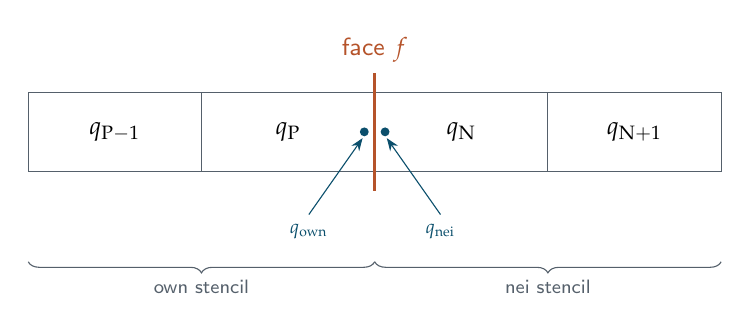
\begin{tikzpicture}[font=\sffamily\small, x=22mm, y=10mm]
  \foreach \i/\lab in {0/P-1, 1/P, 2/N, 3/N+1}{
    \draw[Slate, fill=white] (\i,0) rectangle ++(1,1);
    \node at (\i+0.5,0.5) {$q_{\mathrm{\lab}}$};
  }
  \draw[Rust, very thick] (2,-0.25) -- (2,1.25) node[above] {\color{Rust}face $f$};
  \fill[Ink] (1.94,0.5) circle (1.6pt);
  \fill[Ink] (2.06,0.5) circle (1.6pt);
  \draw[Ink, -{Stealth[length=1.6mm]}] (1.62,-0.55) node[below, font=\sffamily\scriptsize] {$q_\own$} -- (1.93,0.42);
  \draw[Ink, -{Stealth[length=1.6mm]}] (2.38,-0.55) node[below, font=\sffamily\scriptsize] {$q_\nei$} -- (2.07,0.42);
  \draw[decorate, decoration={brace, amplitude=4pt, mirror}, Slate]
      (0,-1.15) -- (2,-1.15) node[midway, below=3pt, font=\sffamily\scriptsize] {own stencil};
  \draw[decorate, decoration={brace, amplitude=4pt, mirror}, Slate]
      (2,-1.15) -- (4,-1.15) node[midway, below=3pt, font=\sffamily\scriptsize] {nei stencil};
\end{tikzpicture}
\caption{Face convention. In Uintah the face index equals the index of cell $N$.}
\end{figure}

\begin{equation}
  q_\own = q_P + \tfrac12\,\psi(r_P)\,(q_N-q_P),\qquad
  r_P = \frac{q_P-q_{P-1}}{q_N-q_P},
\end{equation}
\begin{equation}
  q_\nei = q_N - \tfrac12\,\psi(r_N)\,(q_N-q_P),\qquad
  r_N = \frac{q_{N+1}-q_N}{q_N-q_P}.
\end{equation}
With a central cell gradient on a uniform mesh, OpenFOAM's gradient-based ratio
$r = 2\,(\mathbf d\cdot\nabla q)_P/(q_N-q_P)-1$ reduces to exactly $r_P$ above, so the two
constructions agree. The limiter $\psi(r)$ is zero for $r\le 0$ (a local extremum falls back
to first order), and otherwise:

\begin{center}
\renewcommand{\arraystretch}{1.6}
\begin{tabular}{@{}l l l@{}}
\toprule
\code{limiter=} & $\psi(r),\ r>0$ & note \\
\midrule
\code{vanAlbada} (default) & $\dfrac{r(r+1)}{r^2+1}$ & OpenFOAM definition, used by the reference tutorials \\[1.5ex]
\code{vanLeer}  & $\dfrac{2r}{1+r}$ & \\[1.5ex]
\code{minmod}   & $\min(r,1)$ & most dissipative second-order choice \\
\code{MC}       & $\min\bigl(2r,\ \tfrac{1+r}{2},\ 2\bigr)$ & least dissipative \\
\code{upwind}   & $0$ & first order everywhere \\
\bottomrule
\end{tabular}
\end{center}

\noindent Vector fields are limited component by component. If $|q_N-q_P|$ is at round-off
level, then $q_\own=q_P$ and $q_\nei=q_N$.

\paragraph{Boundaries}
The four-cell stencil needs $P-1$ and $N+1$. Whether they exist is decided from the
\emph{level's} cell index range, including extra cells (\code{Level::findCellIndexRange}) and
periodicity, never from the extent of a fetched array. When $P-1$ (or $N+1$) falls outside,
that side is taken to first order ($\psi=0$). The index substituted for the missing cell is
$P$ (or $N$), so no array is ever indexed out of range: C++ evaluates the arguments before
the call even when their values go unused.

\begin{incode}
\file{Core/CentralUpwind.h} (pure math, no Patch or DataWarehouse): \code{limiter()},
\code{ownNei()} for scalars and \code{Vector}, \code{upwindValue()}.\\
\file{ICE.cc}: file-local \code{ktStencilFlags()}, plus the \code{Pm1Safe/Np1Safe} idiom at every call site.
\end{incode}

%======================================================================
\section{Central-upwind weights and the blending function}\label{sec:weights}
%======================================================================

\subsection{Local wave speeds and the \texorpdfstring{$\alpha$}{alpha} weights}

With $u_\own,u_\nei$ the reconstructed face-normal velocities and $c_\own,c_\nei$ the
reconstructed sound speeds, the one-sided local speeds of propagation are
\begin{equation}
  a^+ = \max\bigl(u_\own+c_\own,\ u_\nei+c_\nei,\ 0\bigr),\qquad
  a^- = \min\bigl(u_\own-c_\own,\ u_\nei-c_\nei,\ 0\bigr).
\end{equation}
\begin{center}
\begin{tabular}{@{}l c c@{}}
\toprule
\code{fluxScheme} & $\alpha_\own$ & $a_{Sf}$ \\
\midrule
\code{Kurganov} (default) & $\dfrac{a^+}{a^+-a^-}$ & $a^-\,\alpha_\own \;\le 0$ \\[2mm]
\code{Tadmor} & $\tfrac12$ & $-\tfrac12\max(a^+,-a^-)$ \\
\bottomrule
\end{tabular}
\end{center}
with $\alpha_\nei = 1-\alpha_\own$. With these, the KT numerical flux of a conserved
quantity $U$ with physical flux $F$ is
\begin{equation}
  \mathcal F_f = \alpha_\own F_\own + \alpha_\nei F_\nei + a_{Sf}\,(U_\nei - U_\own).
  \label{eq:kt}
\end{equation}
Because $a_{Sf}\le 0$, the last term is a dissipation proportional to the jump
between the two reconstructions. In smooth flow the two reconstructions nearly coincide and
the term vanishes; at a shock the limiter opens the jump and the term switches on.
Supersonic flow gives $a^-=0$, so $\alpha_\own=1$ and $a_{Sf}=0$: the flux becomes pure
upwind, from the own side.

\subsection{The hybrid blending function \texorpdfstring{$\kappa$}{kappa}}

reactingPimpleCentralFoam blends between the compressible KT flux and a pressure-based,
upwind-limited flux with
\begin{equation}
  \kappa = \min\!\left(\frac{\mathrm{Ma}_f}{\mathrm{Co}_{ac}},\ 1\right),\qquad
  \mathrm{Ma}_f = \frac{|\alpha_\own u_\own + \alpha_\nei u_\nei|}{\alpha_\own c_\own + \alpha_\nei c_\nei},\qquad
  \mathrm{Co}_{ac} = \frac{\max(a^+,-a^-)\,\dt}{\Delta x_d}
\end{equation}
(\code{kappaFunction MachToAcCourant}, the reference's \emph{standardMachToAcCourantRatio}).
The value \code{kappaFunction one} forces $\kappa=1$. Near a detonation front
$\mathrm{Ma}\sim 1$ and $\mathrm{Co}_{ac}\lesssim 0.5$, so $\kappa=1$ (full KT). In a
low-Mach deflagration $\kappa\ll 1$ and the scheme relaxes toward an upwind-limited flux
close to baseline ICE.

\begin{deviation}
The reference computes $\kappa$ at the end of an outer iteration from the mass fluxes of
that iteration, and uses it in the next. Here $\kappa$ is computed from the reconstructed
cell states at the start of each fluid-chain pass. Inside the outer loop this is equivalent
to a lag of one iteration.
\end{deviation}

\begin{incode}
Task \code{ICE::computeCentralWeights}, scheduled right after the equilibration pressure.
Inputs: \code{rho\_CC}, \code{speedSound\_CC} (NewDW) and \code{vel\_CC} (OldDW), all at ghost 2,
plus \code{delT}. Outputs: \code{ktAlphaOwn\_FC\{X,Y,Z\}}, \code{ktaSf\_FC\{X,Y,Z\}} and
\code{ktKappa\_FC\{X,Y,Z\}}.
\end{incode}

%======================================================================
\section{Split mass fluxes}\label{sec:flux}
%======================================================================

Once ICE has produced the final face velocity $u_f$ for the step (\code{uvel\_FCME} after the
face momentum exchange), the reference's split fluxes are formed:
\begin{align}
  \tilde u_\own &= \alpha_\own u_f - a_{Sf}, &
  \tilde u_\nei &= \alpha_\nei u_f + a_{Sf}, \label{eq:aphiv}\\
  \rho^\kappa_\own &= \kappa\rho_\own + (1-\kappa)\rho_{up}, &
  \rho^\kappa_\nei &= \kappa\rho_\nei + (1-\kappa)\rho_{up}, \\
  \phi_\own &= \tilde u_\own\,\rho^\kappa_\own, &
  \phi_\nei &= \tilde u_\nei\,\rho^\kappa_\nei ,
\end{align}
where $\rho_{up}$ is the own or nei density chosen by the sign of $u_f$, and
$\tilde u_\own$, $\tilde u_\nei$ are the reference's \code{aphiv\_own} and \code{aphiv\_nei}. The
$\kappa$ blend of the densities is the reference's blend of \code{psi\_own/nei} toward a
single face value. Last comes the reference's \code{updateKappa} redistribution:
\begin{equation}
  \phi_\own \leftarrow \phi_\own + (1-\kappa)\,\phi_\nei,\qquad
  \phi_\nei \leftarrow \kappa\,\phi_\nei .
\end{equation}

\paragraph{Two identities worth knowing}
The redistribution leaves the total mass flux $\phi_\own+\phi_\nei$ unchanged. Writing
$\rho_F = \kappa(\alpha_\own\rho_\own+\alpha_\nei\rho_\nei)+(1-\kappa)\rho_{up}$,
\begin{equation}
  \phi_\own+\phi_\nei = \rho_F\,u_f + \kappa\,a_{Sf}\,(\rho_\nei-\rho_\own),
  \qquad\text{so}\qquad
  U_{KT} \equiv \frac{\phi_\own+\phi_\nei}{\rho_F} = u_f + \kappa\,a_{Sf}\,\frac{\rho_\nei-\rho_\own}{\rho_F}.
  \label{eq:ukt}
\end{equation}
So the KT face volume flux is ICE's own face velocity plus an acoustic dissipation that
is proportional to the density jump and switched by $\kappa$. The limits are:
\begin{itemize}
  \item $\kappa=1$: the full KT mass flux, $\alpha_\own\rho_\own u_f + \alpha_\nei\rho_\nei u_f + a_{Sf}(\rho_\nei-\rho_\own)$.
  \item $\kappa=0$: $\phi_\own=\rho_{up}u_f$ and $\phi_\nei=0$, which is TVD upwind transport.
\end{itemize}

\begin{incode}
Task \code{ICE::computeCentralFluxes}, scheduled after the face momentum exchange and before
the pressure update. Outputs: \code{ktPhiOwn\_FC*}, \code{ktPhiNei\_FC*} and \code{ktUvol\_FC*}
($=U_{KT}$).
\end{incode}

%======================================================================
\section{Transport: the CentralUpwind advector}\label{sec:adv}
%======================================================================

ICE advects per-cell extensive quantities $Q_L$ (mass, momentum, internal energy,
the \code{newPressWork} kinetic-energy carrier $K_L$, specific-volume $\times$ mass, and
species mass), and adds the net transfer to $Q_L$. The new advector implements the
reference's \code{fvmDiv(phi\_own, q) + fvmDiv(phi\_nei, q)} with vanAlbada-limited
interpolation:

\begin{equation}
  q = Q_L/m_L,\qquad
  \mathcal F_f = \phi_\own\, q^{\,up}(\phi_\own) + \phi_\nei\, q^{\,up}(\phi_\nei),\qquad
  q^{\,up}(\phi) = \begin{cases} q_\own & \phi\ge 0\\ q_\nei & \phi<0\end{cases}
\end{equation}
\begin{equation}
  \Delta Q_c = \dt\sum_{d} A_d\Bigl(\mathcal F_{f^-_d} - \mathcal F_{f^+_d}\Bigr),
  \qquad Q^{adv}_c = Q_{L,c} + \Delta Q_c .
\end{equation}
Mass is the case $q\equiv 1$. With $\kappa=1$, the transfer of $\rho q$ reproduces the
KT flux~\eqref{eq:kt}: the $a_{Sf}$ parts of $\tilde u_\own,\tilde u_\nei$ carry
$a_{Sf}\bigl((\rho q)_\nei-(\rho q)_\own\bigr)$.

For intensive fields (\code{vol\_frac}, used by the pressure update) the advector uses a
volume flux: $\Delta q_c = \frac{\dt}{V}\sum_d A_d\bigl(q_{f^-}u^\star_{f^-}-q_{f^+}u^\star_{f^+}\bigr)$,
where $q_f$ is the limited upwind value and $u^\star$ is whatever face velocity the caller
passed in (Section~\ref{sec:press}).

\paragraph{Bullet-proofing}
If the outgoing mass of a cell exceeds its Lagrangian mass, or the outgoing volume exceeds
the cell volume, the advector requests a timestep recompute, exactly as the existing
advectors do. AMR refluxing is not supported, and the advector throws if it is requested.

\begin{incode}
\file{Advection/CentralUpwindAdvector.\{h,cc\}}, registered in \file{AdvectionFactory.cc} as type
\code{CentralUpwind} with the \code{limiter} attribute. \code{advectVarBasket} carries the
six $\phi$ arrays. Face transfers are evaluated on demand per face, never cached in a
patch-sized buffer: the face shared with a higher-index neighbour patch is not part of a
patch's own face range (see Section~\ref{sec:lessons}).
\end{incode}

%======================================================================
\section{Face velocity, face pressure and the pressure update}\label{sec:press}
%======================================================================

\subsection{Face velocity (\code{faceVelocity})}
ICE's face velocity is a centred, density-weighted average of the two cell velocities
(\code{term1}), plus a pressure-gradient term (\code{term2}) and gravity. With the flag on,
only the average is replaced, by its KT analogue: the reference's \code{HbyA} interpolated
own/nei and weighted by $\alpha$,
\begin{equation}
  \text{term1} = \alpha_\own\,u_\own + \alpha_\nei\,u_\nei .
\end{equation}
The pressure and gravity terms are unchanged, and the flag-off expression is kept
verbatim.

\subsection{Face pressure (\code{facePressure})}
The reference builds the momentum pressure force as
$\nabla p \approx \mathrm{div}\bigl((\alpha_\own p_\own+\alpha_\nei p_\nei)\,\mathbf S_f\bigr)$.
Correspondingly,
\begin{equation}
  p_f = \alpha_\own\,p_\own + \alpha_\nei\,p_\nei .
\end{equation}
This is an upwind-biased weighted average \emph{without} a jump term. It is not a Riemann
star pressure, which carries an impedance jump $Z_LZ_R(u_L-u_R)/(Z_L+Z_R)$ and adds
dissipation a second time on top of the swept-volume advection.

\paragraph{Energy consistency}
With \code{newPressWork 1}, ICE forms the flow work from \code{press\_FC} and cell-centred
velocities, built term for term to match the momentum pressure source. The KT $p_f$ therefore
feeds momentum and energy consistently, with no further change. The kinetic energy that the
KT momentum transport dissipates is returned as heat by the existing $K_L$ advection
correction, because $K_L$ is advected by the same KT advector.

\subsection{Pressure update (\code{ktPressureFlux})}
In explicit ICE the pressure increment is
$\delta p_{\mathrm{dil}} = -\bigl(\sum_m \dt\,\nabla\!\cdot(\theta_m u_f)\bigr)/\sum_m\kappa_m$,
computed through the advector with the face velocity supplied by the caller. With the flag
on, that velocity is $U_{KT}$ from~\eqref{eq:ukt} instead of $u_f$. The dilatation then
contains the extra term $\kappa\,a_{Sf}(\rho_\nei-\rho_\own)/\rho_F$. This is the explicit
counterpart of the convective part of the reference's pressure equation,
$\mathrm{div}(\phi^d_\own p)+\mathrm{div}(\phi^d_\nei p)$: the KT mass-flux divergence
with its acoustic upwinding.

\begin{deviation}
The reference pressure equation also contains the implicit Laplacian
$-\mathrm{lap}(D_{p,\own},p)-\mathrm{lap}(D_{p,\nei},p)$ and runs \code{nCorrectors} PISO sweeps.
Explicit ICE has no global pressure solve. The closest analogue is the pressure term already
in ICE's face velocity. See Section~\ref{sec:why-explicit} for why this is acceptable for
detonations.
\end{deviation}

%======================================================================
\section{The PIMPLE outer loop}\label{sec:outer}
%======================================================================

\subsection{The update rule}
Let $X$ be any conserved per-cell quantity: mass, momentum, specific volume $\times$ mass,
species mass, or total energy. Write $\mathcal C(\cdot)$ for one pass of the fluid chain,
which maps a starting state to its advected state. The main graph computes
$X^{adv}_0=\mathcal C(X^n)$, and its conversion to primitives is iterate $X^{(0)}$. For
$k=1,\dots,N-1$ the chain is run again from the previous iterate, and the result is combined
with the Crank--Nicolson rule:
\begin{equation}
  \boxed{\;X^{(k)} = X^n + (1-\theta)\bigl(X^{adv}_0 - X^n\bigr) + \theta\bigl(\mathcal C(X^{(k-1)}) - X^{(k-1)}\bigr)\;}
  \label{eq:theta}
\end{equation}
Each bracket is $\dt$ times the fluid-chain tendency, evaluated at $X^n$ and at the latest
iterate respectively. Every quantity inside the chain is therefore re-evaluated at the
latest iterate: the KT weights and $\kappa$, the face velocities, the pressure, the fluxes
and the face states. This matches the reference, which calls \code{updateCentralWeights}
and \code{updateKappa} in every outer iteration. If the iteration converges, the fixed point
is the $\theta$-scheme; $\theta=\tfrac12$ is the tutorial's \code{ddt CrankNicolson 1}.

\paragraph{Two outer iterations are Heun's method}
With $N=2$ and $\theta=\tfrac12$, write $\mathcal C(X)=X+\dt\,\mathcal L(X)$. Then
$X^{(0)}=X^n+\dt\mathcal L(X^n)$ and
\begin{equation}
  X^{(1)} = X^n + \tfrac{\dt}{2}\,\mathcal L(X^n) + \tfrac{\dt}{2}\,\mathcal L\bigl(X^{(0)}\bigr),
\end{equation}
which is the two-stage strong-stability-preserving Runge--Kutta method. Unlike forward
Euler, it keeps the TVD property of the limited spatial operator under a CFL restriction. This
is the most direct reason to expect fewer post-shock oscillations. $\theta=1$ gives a
Picard iteration toward backward Euler.

\paragraph{Energy is blended as total energy}
Blending momentum and internal energy separately would create or destroy heat through the
nonlinearity of $\tfrac12|\mathbf m|^2/M$. Instead, each of the four states
$s\in\{n,\ adv_0,\ \mathcal C,\ k-1\}$ is converted to $E_s = I_s + \tfrac12|\mathbf m_s|^2/M_s$,
$E$ is blended with~\eqref{eq:theta}, and the internal energy is recovered as
$I^{(k)} = E^{(k)} - \tfrac12|\mathbf m^{(k)}|^2/M^{(k)}$. The internal energies at $n$ and $k-1$
are built exactly as the Lagrangian phase builds them: $M\,e_s(T,Y)$ from the model that owns
the caloric equation of state (gasCombustion), or $M c_v T$ otherwise.

\paragraph{Chemistry is evaluated once per step}
As in the reference (\code{reaction->correct()} before \code{pimple.loop()}), the model
sources (chemistry and diffusion) are computed from $u^n$ in the main graph and copied
unchanged into every outer iteration. Because both brackets of~\eqref{eq:theta} contain the
same frozen source, the source enters once, with weight one.

\paragraph{Residual}
After each outer iteration the code reports
$r_k=\max_c\max\bigl(|\rho^{(k)}-\rho^{(k-1)}|/\rho^{(k)},\ |T^{(k)}-T^{(k-1)}|/T^{(k)}\bigr)$,
a global maximum. With \code{outerTolerance}$\,>0$ the loop stops early once
$r_k<$ \code{outerTolerance}. The default is a fixed count, as in the reference.

\subsection{How it is realised in Uintah}

\begin{enumerate}[leftmargin=*]
  \item \textbf{Sub-scheduler.} \code{d\_pimpleSched} is created in \code{problemSetup} with the
        data-warehouse mapping ParentOld$\to$0, ParentNew$\to$1, Old$\to$2, New$\to$3 (coarse = fine
        on a single level). Its graph (Figure~\ref{fig:flow}) is compiled once and recompiled
        whenever the main graph is.
  \item \textbf{Driver task.} \code{pimpleOuterLoop} runs in the main graph right after
        conserved$\to$primitive, \emph{once per processor} (per-processor patch set, as with
        impICE's \code{implicitPressureSolve}), because \code{execute()} of the sub-graph is
        collective.
  \item \textbf{Seeding.} The $k=0$ primitives (\code{rho\_CC}, \code{vel\_CC}, \code{temp\_CC},
        \code{sp\_vol\_CC}, \code{press\_CC}, \code{speedSound\_CC}, \code{specific\_heat}, species)
        are transferred from ParentNewDW into a primed sub-DW. Each iteration then rotates the
        sub-DWs so that the previous iterate becomes the sub-OldDW. \code{delT},
        \code{timeStep} and \code{simTime} are put back in every iteration.
  \item \textbf{Captured advected state.} Right after the main-graph advection, a small task
        copies \code{mass\_adv}, \code{mom\_adv}, \code{eng\_adv}, \code{sp\_vol\_adv} and every
        species \code{var\_adv} into \code{*\_adv0} labels. \code{pimpleBlend} reads $X^{adv}_0$ from
        them, which avoids requiring a label from ParentNewDW while modifying the same label in
        the sub-NewDW.
  \item \textbf{Copy-back.} After the last iteration the primitives (including \code{mach},
        \code{press\_CC} and species) are copied into ParentNewDW over \emph{extra cells too},
        so the next step starts from the final iterate's boundary values as well as its
        interior values.
  \item \textbf{Timestep control.} A recompute or abort request raised inside the sub-graph is
        forwarded to the main graph.
\end{enumerate}

\begin{incode}
\file{ICE.cc} (each with its \code{schedule...} pair):\\
\hspace*{1em}\code{pimpleOuterLoop}, \code{capturePimpleAdv0}, \code{pimpleCopyModelSources},\\
\hspace*{1em}\code{pimpleBlend}, \code{pimpleResidual}.\\
\file{Core/ICELabel.*}: \code{mass\_adv0}, \code{mom\_adv0}, \code{eng\_adv0}, \code{sp\_vol\_adv0},
\code{pimpleResidual}.\\
Per-iteration residual print: \code{SCI\_DEBUG="ICE\_PIMPLE:+"}.
\end{incode}

\subsection{Why explicit ICE is enough for detonations}\label{sec:why-explicit}
pimpleCentralFoam is pressure-implicit so that it can take acoustic Courant numbers
$\gg 1$ at low Mach, where $\kappa\to 0$ and the scheme becomes pressure-based. In the
detonation tutorials, \code{maxCo 0.1} keeps $\mathrm{Co}_{ac}\approx 0.1$--$0.3$ at the front,
so $\kappa=1$ and the implicit Laplacian is a small correction. A large implicit step would
push $\kappa$ toward zero and smear the shock and the induction zone. The stability that
matters here comes from the KT dissipation and the TVD time integration, both of which the
explicit version has. An impICE variant would pay off only for runs that also need long,
low-Mach phases, such as deflagration-to-detonation transition.

%======================================================================
\clearpage
\section{Fidelity map}
%======================================================================

\begin{center}
\small
\renewcommand{\arraystretch}{1.25}
\begin{tabularx}{\linewidth}{@{}>{\raggedright\arraybackslash}X >{\raggedright\arraybackslash}X@{}}
\toprule
\textbf{reactingPimpleCentralFoam} & \textbf{Uintah ICE (this work)} \\
\midrule
\code{reconstruct(rho, U, p, psi)}, own/nei, vanAlbada & \code{centralUpwind::ownNei}, default limiter vanAlbada \\
\code{ap}, \code{am}, \code{alpha\_own}, \code{aSf} (Kurganov / Tadmor) & \code{computeCentralWeights} \\
\code{kappa} (standardMachToAcCourantRatio) & \code{computeCentralWeights}; $\kappa$-blend and redistribution in \code{computeCentralFluxes} \\
\code{aphiv\_own/nei}, \code{phi\_own/nei}, \code{updateKappa} & \code{computeCentralFluxes} \\
\code{fvmDiv(phi\_own,$\cdot$)+fvmDiv(phi\_nei,$\cdot$)} for U, Y, h & \code{CentralUpwindAdvector} (mass, momentum, $I$, $K_L$, specific volume, species) \\
\code{gradp} with $\alpha$-weighted $p_\own,p_\nei$ & \code{computePressFC} (\code{facePressure}) \\
\code{HbyA} interpolated own/nei with $\alpha$ & \code{computeVelFace} term1 (\code{faceVelocity}) \\
pEqn convective terms $\mathrm{div}(\phi^d p)$ & $U_{KT}$ in the explicit pressure update (\code{ktPressureFlux}) \\
pEqn Laplacian, \code{nCorrectors} & not implemented (would need impICE) \\
\code{reaction->correct()} once per step & model sources once per step, frozen in the outer iterations \\
\code{pimple.loop()}, \code{nOuterCorrectors} & \code{pimpleOuterLoop} sub-scheduler \\
\code{ddt CrankNicolson 1} & $\theta$ rule~\eqref{eq:theta}, $\theta=0.5$ \\
\code{hEqn} (sensible enthalpy, KChange, KSource) & ICE internal energy with \code{newPressWork 1}; total-energy blend in the loop \\
\code{maxCo 0.1} & \code{<cfl>} in the input (0.1 in the detonation input) \\
\bottomrule
\end{tabularx}
\end{center}

\begin{deviation}[s, collected]
\begin{itemize}[leftmargin=*]
  \item $\kappa$ is lagged by one outer iteration relative to the reference (Section~\ref{sec:weights}).
  \item Transport inside one outer iteration is explicit, where OpenFOAM assembles implicit
        \code{fvm} matrices. The outer iterations supply the implicit coupling.
  \item There is no implicit pressure Laplacian and no PISO \code{nCorrectors}.
  \item Diffusion is frozen with chemistry across outer iterations. The reference re-solves
        diffusion inside \code{YEqn}/\code{hEqn}.
  \item Energy is carried as internal energy, not sensible enthalpy.
\end{itemize}
\end{deviation}

%======================================================================
\clearpage
\section{Input reference}
%======================================================================

\begin{center}
\small
\renewcommand{\arraystretch}{1.2}
\begin{tabularx}{\linewidth}{@{}l l X@{}}
\toprule
\textbf{Tag} & \textbf{Default} & \textbf{Meaning} \\
\midrule
\multicolumn{3}{@{}l}{\sffamily\color{Ink}\code{<CFD><ICE><advection type="CentralUpwind" limiter="...">}}\\
\code{limiter} & \code{vanAlbada} & vanAlbada, vanLeer, minmod, MC, upwind \\
\midrule
\multicolumn{3}{@{}l}{\sffamily\color{Ink}\code{<CFD><ICE><CentralUpwind>} (optional; requires the advection type above)}\\
\code{fluxScheme} & \code{Kurganov} & or \code{Tadmor} \\
\code{kappaFunction} & \code{MachToAcCourant} & or \code{one} ($\kappa\equiv 1$) \\
\code{faceVelocity} & \code{true} & KT term1 in the face velocity \\
\code{facePressure} & \code{true} & $\alpha$-weighted face pressure \\
\code{ktPressureFlux} & \code{true} & $U_{KT}$ in the pressure update \\
\midrule
\multicolumn{3}{@{}l}{\sffamily\color{Ink}\code{<CFD><ICE><PIMPLE>} (optional)}\\
\code{nOuterCorrectors} & \code{1} & total passes per step; 1 = loop off; the reference uses 2 \\
\code{theta} & \code{0.5} & $\theta$ in~\eqref{eq:theta}; $0<\theta\le 1$ \\
\code{outerTolerance} & \code{0} & 0 = fixed count; otherwise early exit on $r_k$ \\
\code{nCorrectors} & \code{1} & parsed, reserved for an impICE variant \\
\bottomrule
\end{tabularx}
\end{center}

\paragraph{Enforced at start-up}
The outer loop requires explicit ICE, one level, one ICE material and no turbulence model.
CentralUpwind requires one ICE material and no MPM materials; AMR refluxing is rejected at run time.

\paragraph{Provided inputs} In \file{StandAlone/inputs/ICE/RX\_MODELS/}:
\begin{itemize}
  \item \code{cvHydrogen1\_pimple.ups}, \code{hydrogenFlame1\_pimple.ups}: the base cases with KT and PIMPLE
        ($N=2$, $\theta=0.5$). Each also has a \code{\_smoke} copy capped at 200 steps;
        flags-off \code{\_smoke} copies of the originals exist too.
  \item \code{hydrogenShocktube\_pimple.ups}: a gasCombustion detonation in the shock-fixed frame,
        initialised from \code{shockProfile.dat}, with KT, PIMPLE and \code{cfl 0.1}. It saves
        $\kappa$ and $\alpha$ on the $x$ faces.
  \item \code{hydrogenShocktube\_gc\_baseline.ups}: the same case with \code{SecondOrder}
        advection, for A/B comparison.
\end{itemize}

%======================================================================
\section{Suggested checks}
%======================================================================

\begin{enumerate}[leftmargin=*]
  \item \textbf{Oscillations.} Compare \code{nOuterCorrectors} 1 and 2 with everything else
        fixed. This isolates the effect of the time integration from that of the flux.
  \item \textbf{Induction zone.} If it shortens or collapses, first set
        \code{facePressure false}. A dissipative face pressure applied as a cell-centred
        source is the known way to over-dissipate ICE's momentum equation. Then compare
        \code{ktPressureFlux true/false}.
  \item \textbf{Blending.} Compare \code{kappaFunction one} with \code{MachToAcCourant}. The
        detonation front should already sit at $\kappa=1$; inspect \code{ktKappa\_FCX}.
  \item \textbf{Limiter.} Compare minmod, vanAlbada and MC to bracket limiter sensitivity.
  \item \textbf{Time rule.} Compare $\theta=0.5$ with $\theta=1$, and use \code{nOuterCorrectors 3} to check
        the convergence of the residual $r_k$ with \code{SCI\_DEBUG="ICE\_PIMPLE:+"}.
  \item \textbf{Regression.} Remove all new tags. The original code paths should reproduce
        the pre-change results.
\end{enumerate}

%======================================================================
\section{Implementation lessons}\label{sec:lessons}
%======================================================================

Five defects surfaced during testing. Each is a general Uintah pitfall and is recorded
here so it is not rediscovered.

\begin{description}[style=nextline, leftmargin=6mm, font=\sffamily\bfseries\color{Ink}]
  \item[Out-of-range stencil arguments]
        Passing \code{q[Pm1]} to a function that ignores it when the stencil is invalid still
        reads that memory, and at a domain edge with one extra cell this segfaulted. The fix is
        to substitute $P$ or $N$ before indexing (\code{Pm1Safe}/\code{Np1Safe}).
  \item[Patch-sized face buffers]
        \code{Patch::getSFC*HighIndex()} includes the upper face only when the patch has no
        neighbour there. A face buffer filled over a patch's own face range therefore lacks
        the face $c+1$ of the patch's last cell at an interior patch boundary. Reading it gave
        negative specific volume at every patch seam of the 12-rank flame run. Face transfers
        are now evaluated on demand from ghosted data.
  \item[Sub-scheduler driver scheduled per patch]
        A task that calls a sub-scheduler's collective \code{execute()} must be added on the
        per-processor patch set. On \code{level->eachPatch()} it ran once per patch, each time
        with only one patch seeded. This failed as soon as a rank owned more than one patch
        (4 ranks, 12 patches), and went unnoticed with one patch per rank.
  \item[Copy-back over interior cells only]
        The outer loop's final state has to be copied over extra cells too. Otherwise
        the next step's boundary values come from iteration $k=0$, which matters for
        LODI and Neumann boundaries.
  \item[Limiter overflow (found in 2D)]
        The textbook vanAlbada and vanLeer forms, $r(r+1)/(r^2+1)$ and $2r/(1+r)$, evaluate
        $\infty/\infty=\mathrm{NaN}$ when $r$ is huge. That happens when the jump across a face is
        tiny next to a finite upwind jump, which is routine for trace species on an oblique 2D
        front. A 2D channel detonation crashed with NaN temperatures after four steps. For $r>1$
        the code now uses the equivalent forms $(1+1/r)/(1+1/r^2)$ and $2/(1+1/r)$.
\end{description}

%======================================================================
\section*{File index}
\addcontentsline{toc}{section}{File index}
%======================================================================
\begin{center}
\small
\begin{tabularx}{\linewidth}{@{}l X@{}}
\toprule
\file{ICE/Core/CentralUpwind.h} & limiters, own/nei reconstruction, KT weights, $\kappa$ (new) \\
\file{ICE/Advection/CentralUpwindAdvector.\{h,cc\}} & KT transport (new) \\
\file{ICE/Advection/Advector.h} & basket extended with the $\phi$ arrays \\
\file{ICE/Advection/AdvectionFactory.cc}, \file{sub.mk} & registration, \code{limiter} attribute \\
\file{ICE/ICE.\{h,cc\}} & flags, \code{scheduleFluidChain}, KT tasks, face velocity and pressure, pressure update, outer loop \\
\file{ICE/Core/ICELabel.\{h,cc\}} & \code{kt*\_FC*}, \code{*\_adv0}, \code{pimpleResidual} labels \\
\file{StandAlone/inputs/UPS\_SPEC/ice\_spec.xml} & new tags \\
\file{ICE/PIMPLE\_KT.md} & short usage note \\
\bottomrule
\end{tabularx}
\end{center}

\end{document}
